\onecolumn
\chapter{Auswertung}
\label{ch:auswertung}

\section*{Fehlerrechnung}
Für die statistische Auswertung von $n$ Messwerten $x_i$ werden folgende Größen definiert \cite{errorSkript25}:
\begin{align}
    \bar{x} &= \frac{1}{n} \sum_{i=1}^{n} x_i \vphantom{\sqrt{\sum_i^n}^2} && \text{\textcolor{gray}{Arithmetisches Mittel}} \label{eq:arithmetisches_mittel} \\
    \sigma^2 &= \frac{1}{n-1} \sum_{i=1}^{n} (x_i - \bar{x})^2 \vphantom{\sqrt{\sum_i^n}^2} && \text{\textcolor{gray}{Variation}} \label{eq:variation} \\
    \sigma &= \sqrt{\frac{1}{n-1} \sum_{i=1}^{n} (x_i - \bar{x})^2} \vphantom{\sqrt{\sum_i^n}^2} && \text{\textcolor{gray}{Standardabweichung}} \label{eq:standardabweichung} \\
    \Delta \bar{x} &= \frac{\sigma}{\sqrt{n}} = \sqrt{\frac{1}{n(n-1)} \sum_{i=1}^n(\bar x - x_i)^2} \vphantom{\sqrt{\sum_i^n}^2} && \text{\textcolor{gray}{Fehler des Mittelwerts}} \label{eq:fehler_mittelwert} \\
    \Delta f &= \sqrt{\left(\frac{\partial f}{\partial x} \Delta x\right)^2 + \left(\frac{\partial f}{\partial y} \Delta y\right)^2} \vphantom{\sqrt{\sum_i^n}^2} && \text{\textcolor{gray}{Gauß’sches Fehlerfortpflanzungsgesetz für $f(x,y)$}} \label{eq:gauss_fehlfortpflanzung} \\
    \Delta f &= \sqrt{(\Delta x)^2 + (\Delta y)^2} \vphantom{\sqrt{\sum_i^n}^2} && \text{\textcolor{gray}{Fehler für $f = x + y$}} \label{eq:fehler_summe} \\
    \Delta f &= |a| \Delta x \vphantom{\sqrt{\sum_i^n}^2} && \text{\textcolor{gray}{Fehler für $f = ax$}} \label{eq:fehler_proportional} \\
    \frac{\Delta f}{|f|} &= \sqrt{\left(\frac{\Delta x}{x}\right)^2 + \left(\frac{\Delta y}{y}\right)^2} \vphantom{\sqrt{\sum_i^n}^2} && \text{\textcolor{gray}{relativer Fehler für $f = xy$ oder $f = x/y$}} \label{eq:relativer_fehler} \\
    \sigma &= \frac{|a_{lit} - a_{gem}|}{\sqrt{\Delta a_{lit}^2 + \Delta a_{gem}^2}} \vphantom{\sqrt{\sum_i^n}^2} && \text{\textcolor{gray}{Berechnung der signifikanten Abweichung}} \label{eq:signifikante_abweichung}
\end{align}

\twocolumn

% ////////////  Aufgaben Wechsel ////////////
\section{Aufgabe 1: Function Generator}

% ////////////  Aufgaben Wechsel ////////////
\section{Aufgabe 2: Analyse der 9 Signale}

Wir wollen die Signale 1 und 2 genauer analisieren. Signale 3 und 4 werden nur kurz beschrieben. Bei Signal 5 wird die Halbwertszeit berechnet. Signale 7 bis 9 werden dann wieder qualitativ beschrieben.
\subsection*{Signal 1}
\begin{figure} [h!]
    \centering
        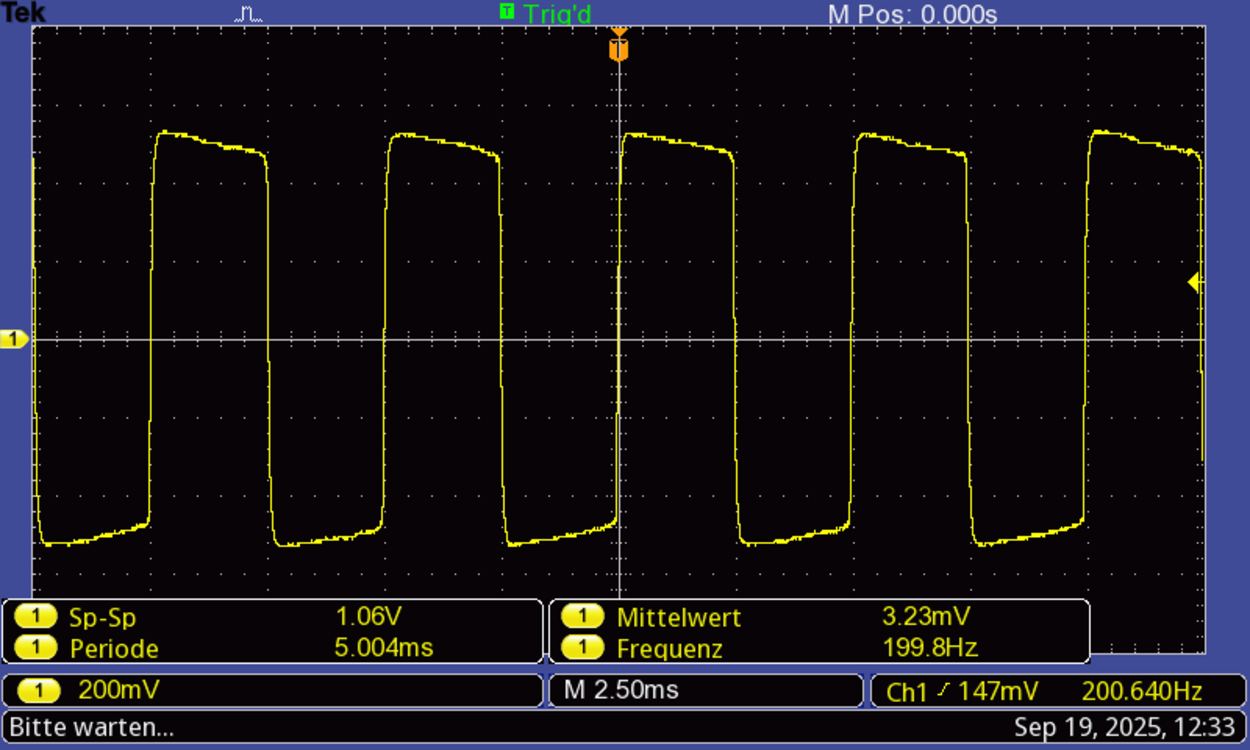
\includegraphics[width=0.45\textwidth]{img/25/Signale2/Signal1-Messwerte.pdf}
    \caption{Signal 1 mit automatischen Messwerten und gesetzem Trigger im AC Modus.}
\end{figure}
Wir mussten zur Vermessung des Signales 1 sowohl manuell mit den Cursorn vermessen und automatisch mit den eingebauten Messfunktionen des Oszilloskopes.
Wir haben dabei eine DIV größe von $200mv \times 2,5ms$ im AC-Modus geahbt und $500mv \times 2,5ms$ im DC-Modus. Aus \hyperref[tab:all_fehler]{Tabelle \ref*{tab:all_fehler}} lassen sich somit die Fehler ablesen beziehungsweise aus den Angaben berechenn lassen zu:
\begin{align}
    &\textcolor{teal}{\Delta V_{AC}} &&= 15\, &&[mV] \\
    &\textcolor{purple}{\Delta V_{DC}} &&= 40\, &&[mV] \\
    &\Delta t &&= 0,16 \, &&[ms].
\end{align}
(Es wurde auf signifikante Stellen gerundet).

In den Tabellen werden die Spalten \textcolor{teal}{Grün} angezeigt, wenn sie in AC gemessen wurden und \textcolor{purple}{Lila}, wenn sie im DC-Modus gemessen wurden. Dies ist nur für die Cursor wichtig.

\begin{figure} [h!]
    \centering
        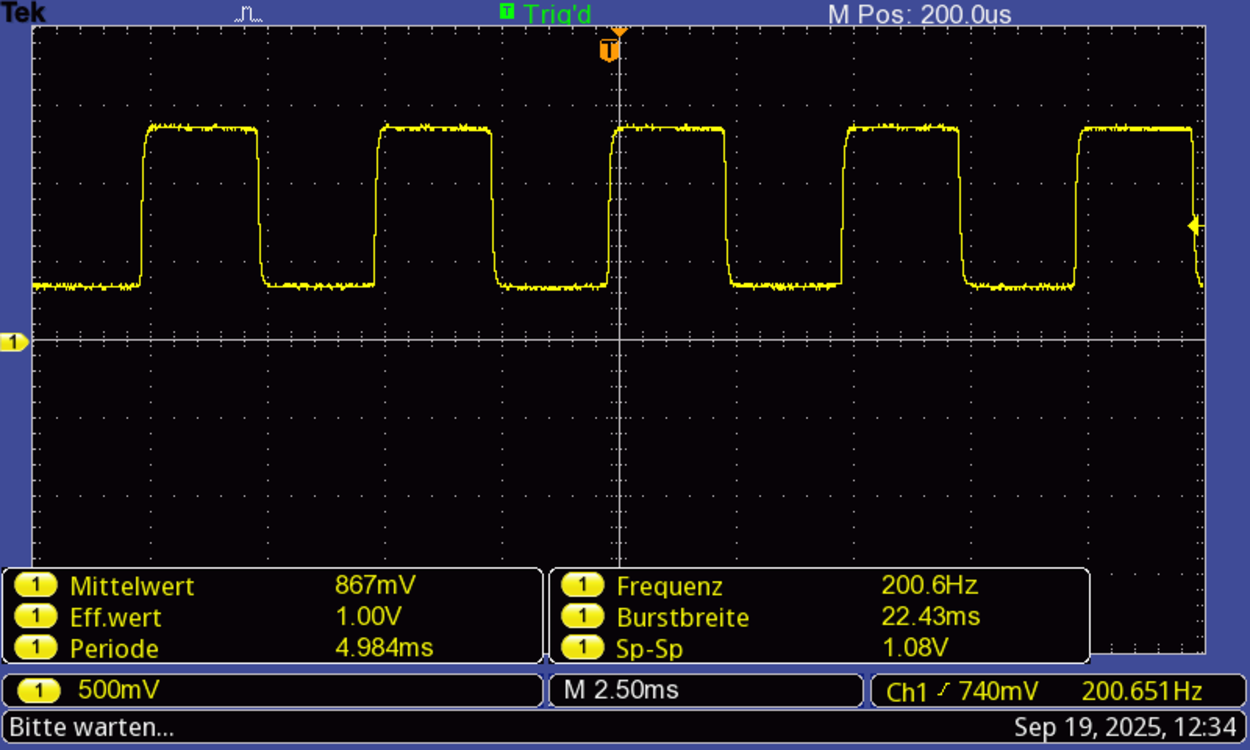
\includegraphics[width=0.45\textwidth]{img/25/Signale2/Signal1-DC.pdf}
    \caption{Signal 1 mit automatischen Messwerten und gesetzem Trigger im DC Modus.}
\end{figure}

Diese Unsicherheiten verwenden wir nun, wenn immer wir Cursor-Messungen zur Berechnung benutzen. Die automatischen Werte sollen als >>perfekt<< angenommen werden.
In den Tabellen beschreibt $T$ die Periodendauer in ms, $U_{SS}$ die Spitzen-Spitze-Spannung (also die Differenz von $U_{max}$ und $U_{min}$). $U_{max}$ und $U_{min}$ sind die lokalen\footnote{Also die auf dem Display angezeigten Extrempunkte.} Extrempunkte. $U_{G}$ ist die $DC_{offset}$-Spannung. Berechnet wird dieser über den Mittelwert im DC-Modus.

Wir schreiben daher einmal alle Informationen aus dem  \hyperref[Protokoll]{Protokoll} in zwei Tabellen, in eine für die automatisch berechneten Werte und eine für die Cursor-Messungen.

\begin{table}[h!]
    \centering
    \begin{tabular}{c | c | c | c | c }
        \toprule
        T [ms] & $U_{SS}$ [V] & $U_{G}$ [V] & $U_{max}$ [V] & $U_{min}$ [V] \\
        \hline
        4,983 & 1,06 & 0,93 & 1,50 & 0,40 \\
        \bottomrule
    \end{tabular}
    \caption{Tabelle der vom Osziloskop berechneten Werte.}
    \label{tab:sig1_auto}
\end{table}

In \hyperref[tab:sig1_auto]{Tabelle \ref*{tab:sig1_auto}} sind alle automatisch gemessenen Werte eingetragen. 

Aus der Periodendauer können wir nun die \hyperref[eq:freq]{Frequenz (\ref*{eq:freq})} berechnen:
\begin{equation}
    \boxed{
        f_{auto} = 0,202 ms^{-1} \, \hat = \, 4,95 kHz
    }.
\end{equation}

Aus den Extrema können wir $U_G$ auch noch rechnerisch über das \hyperref[eq:arithmetisches_mittel]{arithmetische Mittel \ref*{eq:arithmetisches_mittel}} bestimmen:
\begin{equation}
    U_{G,auto,r} = 0,95 V.
\end{equation}

Merkwürdig ist, dass die Werte $U_G$ und $U_{G,auto,r}$ einwenig abweichen. Dies liegt daran, dass das Signal nicht konstant war. Aus nicht bekannten Gründen sind die Werte über die Zeit angestiegen. Da wir die Werte aber nacheinander abgeschrieben haben, waren zu dem Moment die Werte schon nicht mehr stringent. Die Abweichung ist jedoch nicht besonders groß.

\begin{table}[h!]
    \centering
    \begin{tabular}{c | c | c | c }
        \toprule
        T [ms] & \textcolor{teal}{$U_{SS}$ [V]} & \textcolor{purple}{$U_{max}$ [V]} & \textcolor{purple}{$U_{min}$ [V]} \\
        \hline
        $5,00 \pm 0,16 $ & $1,064$ & $1,500$ & $0,460$ \\
        \bottomrule
    \end{tabular}
    \caption{Tabelle der mit Cursor bestimmten Werte. }
    \label{tab:sig1_cursor}
\end{table}

Wir wollen nun $U_{G}$ bestimmen. Dies ist der \hyperref[eq:arithmetisches_mittel]{Mittelwert \ref*{eq:arithmetisches_mittel}} von $U_{max}$ und $U_{min}$. 
\begin{equation}
    U_{G} = 0,980 V.
\end{equation}

Dabei entspricht $U_{G}$ gerade dem Gleichspannungsanteil.

Seinen Fehler bestimmen wir via \hyperref[eq:gauss_fehlfortpflanzung]{Gauß'scher Fehlerfortpflanzung (\ref*{eq:gauss_fehlfortpflanzung})}:
\begin{equation}
    \Delta U_{G} = \sqrt{\left(\Delta U_{min}\right)^2 + \left(\Delta U_{max}\right)^2}.
\end{equation}

Somit kommen wir auf ein Ergebnis von 
\begin{equation}
    \boxed{
        U_{G} = (980 \pm 60) \, mV
    }.
\end{equation}

Als nächstes berechnen wir die Frequenz der Cursor-Messung:
\begin{equation}
    \underline{
        f_{cursor} = 0,2 ms^{-1} \, \hat= \, 5kHz
    }.
\end{equation}

Den Fehler der Frequenz müssen wir noch bestimmen, wieder über \hyperref[eq:gauss_fehlfortpflanzung]{Gauß'scher Fehlerfortpflanzung (\ref*{eq:gauss_fehlfortpflanzung})}:
\begin{equation}
    \Delta f = \frac{\Delta T}{T^2}.
    \label{eq:f_freq}
\end{equation}

Berechenn wir diesen Fehler und tragen das Ergebnis zusammen, kommen wir zu: 
\begin{equation}
    \boxed{
        f_{cursor} = (0,200 \pm 0,006) ms^{-1}
    }.
\end{equation}
(Es wurde auf signifikante Stellen gekürzt.)


Nocheinmal die Gefragten Werte zusammengetragen:
\begin{align*}
    U_{G,auto} &= 930 mV \\
    U_{G,auto,r} &= 0,95 V \\
    U_{SS} &= 1,06 V \\
    f_{auto} &= 0,202 ms^{-1} \\
    \\
    U_{G,cursor}& = (980 \pm 60)\, mV \\
    U_{SS,cursor} &= (1\,064 \pm 15)\, mV \\
    U_{SS,cursor,r} &= (1\,040 \pm 60)\, mV \\
    f_{cursor} &= (0,200 \pm 0,006)\, ms^{-1}
\end{align*}

Der Wert $U_{SS,cursor,r}$ ist dabei der nochmal neu gerechtete Wert, aus dem Maximum und dem Minimum. 

Wir berechnen nun noch, wie signifikant die Werte des Cursors sind, indem wir die autoamtisch berechneten als Referent nehmen. Wir nuzen \hyperref[eq:signifikante_abweichung]{Gleichung \ref*{eq:signifikante_abweichung}} der Fehlerrechnung:
Wir beginnen mit der Offset-Spannung $U_G$:
\begin{equation}
    \frac{\left| U_{G,auto} - U_{G,cursor} \right|}{\Delta U_{G,cursor}} = 0,83\sigma.
\end{equation}

Für die Spitzen-Spitzen-Spannung:
\begin{equation}
    \frac{\left| U_{SS,auto} - U_{SS,cursor} \right|}{\Delta U_{SS,cursor}} = 17\sigma.
\end{equation}

Und zuletzt für die Frequenz:
\begin{equation}
    \frac{\left| f_{auto} - f_{cursor} \right|}{\Delta f_{cursor}} = 0,33\sigma.
\end{equation}


% \begin{figure} [h!]
%     \centering
%         
\includegraphics[width=0.35\textwidth]{img/25/memes/kommunismus.pdf}
%     \caption{Meme nach Signal 1}
% \end{figure}


% ------------------- Signal 2 -------------------

\subsection*{Signal 2}
\begin{figure} [h!]
    \centering
        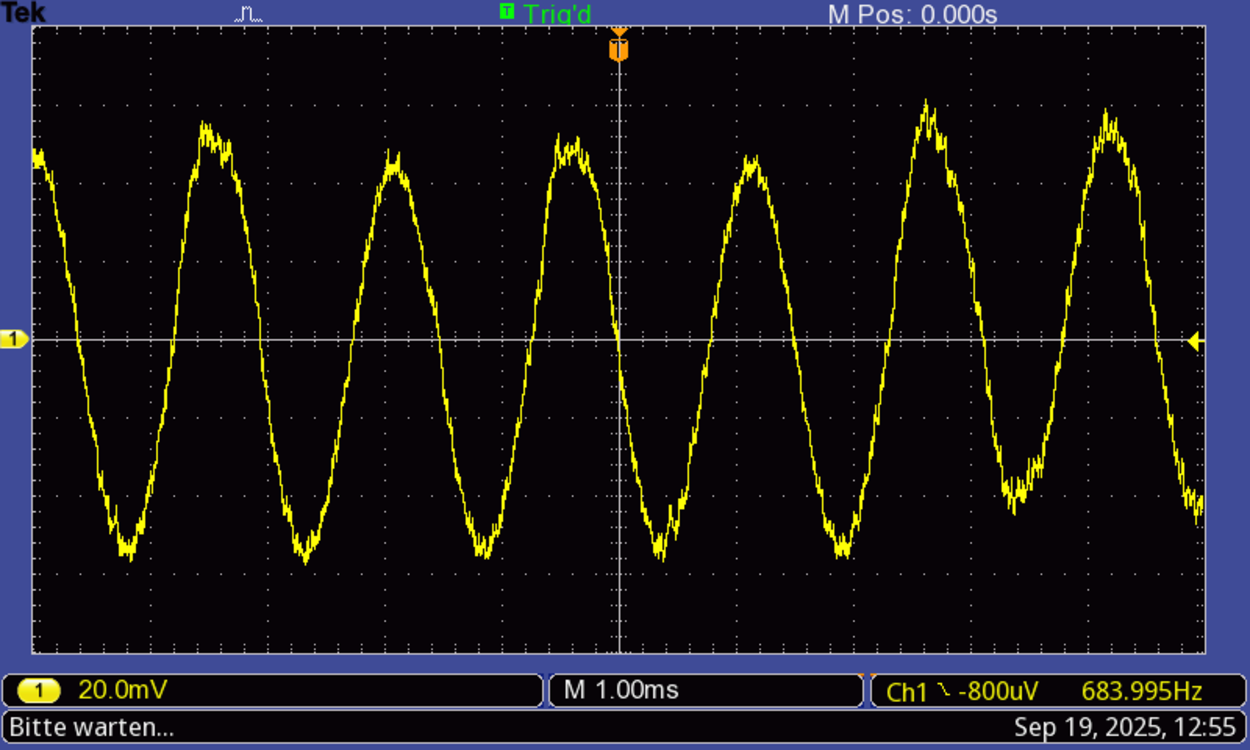
\includegraphics[width=0.45\textwidth]{img/25/Signale2/Signal2-Clean.pdf}
    \caption{Signal 2 mit gesetzem Trigger.}
\end{figure}

Wir schauen uns nun das zweite Signal an, dessen Punkte wir gemessen haben. Die Tabellen sind hier wie bei Signal 1 Aufgebaut.

\begin{table}[h!]
    \centering
    \begin{tabular}{c | c | c | c | c }
        \toprule
        T & $U_{SS}$ [V] & $U_{G}$ [V] & $U_{max}$ [V] & $U_{min}$ [V] \\
        \hline
        --- & 0,104 & 1,61 & -1,56 & -1,67 \\
        \bottomrule
    \end{tabular}
    \caption{Tabelle der vom Osziloskop berechneten Werte des zweiten Signals.}
    \label{tab:sig2_auto}
\end{table}

Die Periodendauer konnte automatisch nicht gemessen werden. Dies lag an dem stark rauschendem (beziehungsweise nicht konstanen) Signal. Auch wenn man es pausiert, kann keine automatische Periodenmessung stattfinden. Als logische Konsequenz kann hier keine Frequenz bestimmt werden.

Neben den automatisch berechneten Werten für $U_{SS}$ und $U_G$ wollen wir die Rechnung über die $U_{max}$ und die $U_{min}$ nochmal überprüfen:
\begin{equation}
    U_{SS,r} = 0,11 V,
\end{equation}
\begin{equation}
    U_{G,r} = 1,615 V.
\end{equation}

Es sind leichte Abweichungen zu erkennen, aber grundsätzlich sind die Werte stringent. Die Abweichungen kommen wie bei Signal 1 daher, dass die Signale nicht kontinuirlich sind, sonder Schwankungen unterliegen. 

Für die Cursor-Messung müssen wir zunächst wieder die Fehler bestimmen. Wir haben dieses mal für die AC-Spannung ein Step-Grid von $20mv \times 1,00ms$. Für die DC-Spannung $50mv \times 1,00ms$. Wir greifen wieder auf die \hyperref[tab:all_fehler]{Tabelle \ref*{tab:all_fehler}} zurück und kommen somit auf Ungenauigkeiten von:
\begin{align}
    \Delta t &= 0,006 ms \\
    \textcolor{teal}{\Delta U_{AC}} &=1,5 mV \\
    \textcolor{purple}{\Delta U_{DC}} &= 4,0 mV
\end{align}

Wir tragen nun die Werte der Messungen in die Tabelle ein:
\begin{table}[h!]
    \centering
    \begin{tabular}{c | c | c | c }
        \toprule
        T [ms] & \textcolor{teal}{$U_{SS}$ [mV]} & \textcolor{purple}{$U_{max}$ [mV]} & \textcolor{purple}{$U_{min}$ [mV]} \\
        \hline
        $1,560$ & $125,6$ & $68,8$ & $56,8$ \\
        \bottomrule
    \end{tabular}
    \caption{Tabelle der mit Cursor bestimmten Werte. }
    \label{tab:sig2_cursor}
\end{table}

Wir berechen die \hyperref[eq:freq]{Frequenzen (\ref*{eq:freq})} Cursor- Messung:
\begin{equation}
    f_{cursor} = 0,641 ms^{-1}.
\end{equation}

Sein Fehler wird Analog zu \hyperref[eq:f_freq]{Gleichung \ref*{eq:f_freq}} berechnet. Wir kommen also auf ein Ergebnis von
\begin{equation}
\boxed{
    f = (0,6410 \pm 0,0025) \, ms^{-1}
}.
\end{equation}

Als nächstes wollen wir $U_G$ aus der Cursor-Messung bestimmen. Diese ist wieder Analog zum ersten Signal. 
Unser $U_{G,cursor}$ ist somit:
\begin{equation}
    U_{G,cursor} = 62,8 mV,
\end{equation}
mit einer Ungenauigkeit von
\begin{equation}
    \Delta U_{G,cursor} = 5,657 mV.
\end{equation}

Als Ergebnis also:
\begin{equation}
\boxed{
    U_{G,cursor} = (63 \pm 6) \, mV
}
\end{equation}

Recht offensichtlich ist der gemessene Wert der $U_{SS}$-Spannung nicht richtig. Wir würden eigentlich erwarten:
\begin{equation}
    U_{SS,r} = 12 mV
\end{equation}

Der oben angegebene Wert ist scheinbar einfach die Summe der Extrema. Diese Berechnung ist flasch. Wir haben diesen Wert hier also offensichtlich nicht gemessen, sondern falsch berechnet. Von nun an ist $U_{SS,r}$ der richtige Wert.
Wir müssen seine Ungenauigkeit noch bstimmen. Diese ist jedoch einfach identisch zur $U_G$-ungenauigkeit. Unser Ergebnis ist somit:
\begin{equation}
    \boxed{
        U_{SS,cursor} = (12 \pm 6) mV.
    }
\end{equation}



\newpage
\onecolumn
\twocolumn

% ------------------- Signal 3 -------------------
\subsection*{Signal 3}
\begin{figure} [h!]
    \centering
        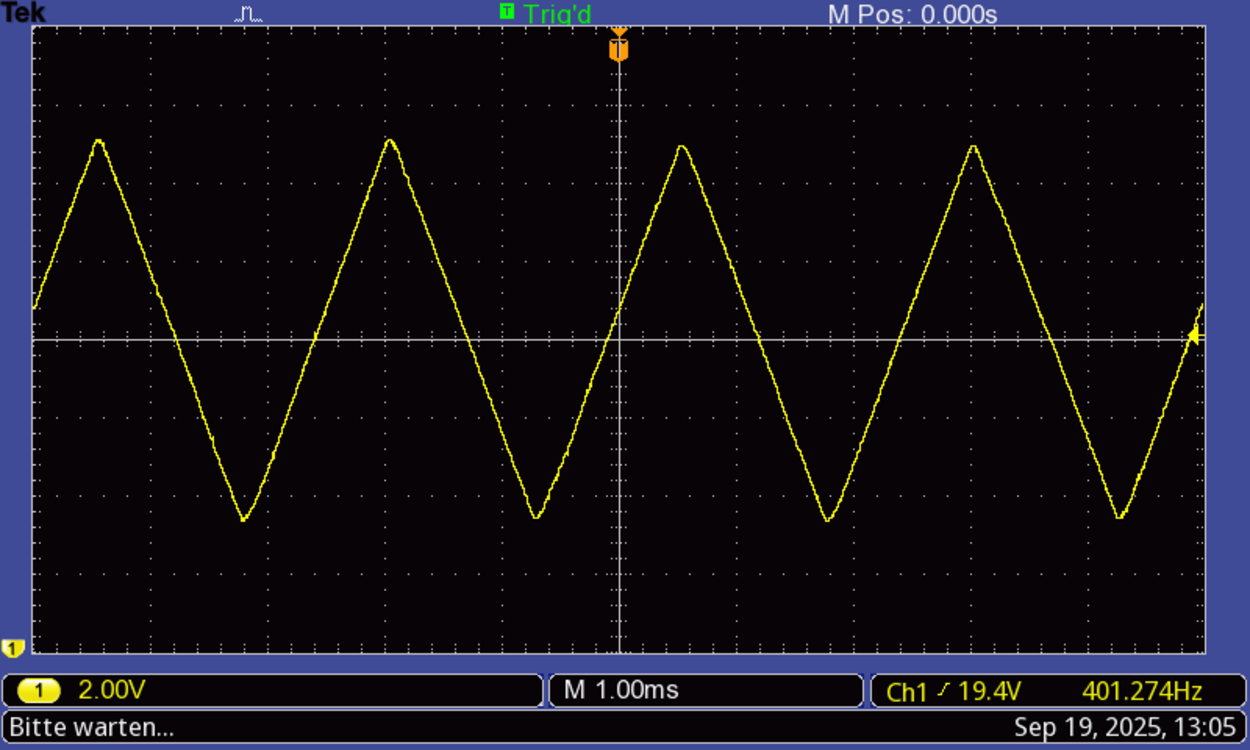
\includegraphics[width=0.45\textwidth]{img/25/Signale2/Signal3.pdf}
    \caption{Signal 3}
\end{figure}

Signal 3 ist ein Zick-Zack-Signal.

% ------------------- Signal 4 -------------------
\subsection*{Signal 4}
\begin{figure} [h!]
    \centering
        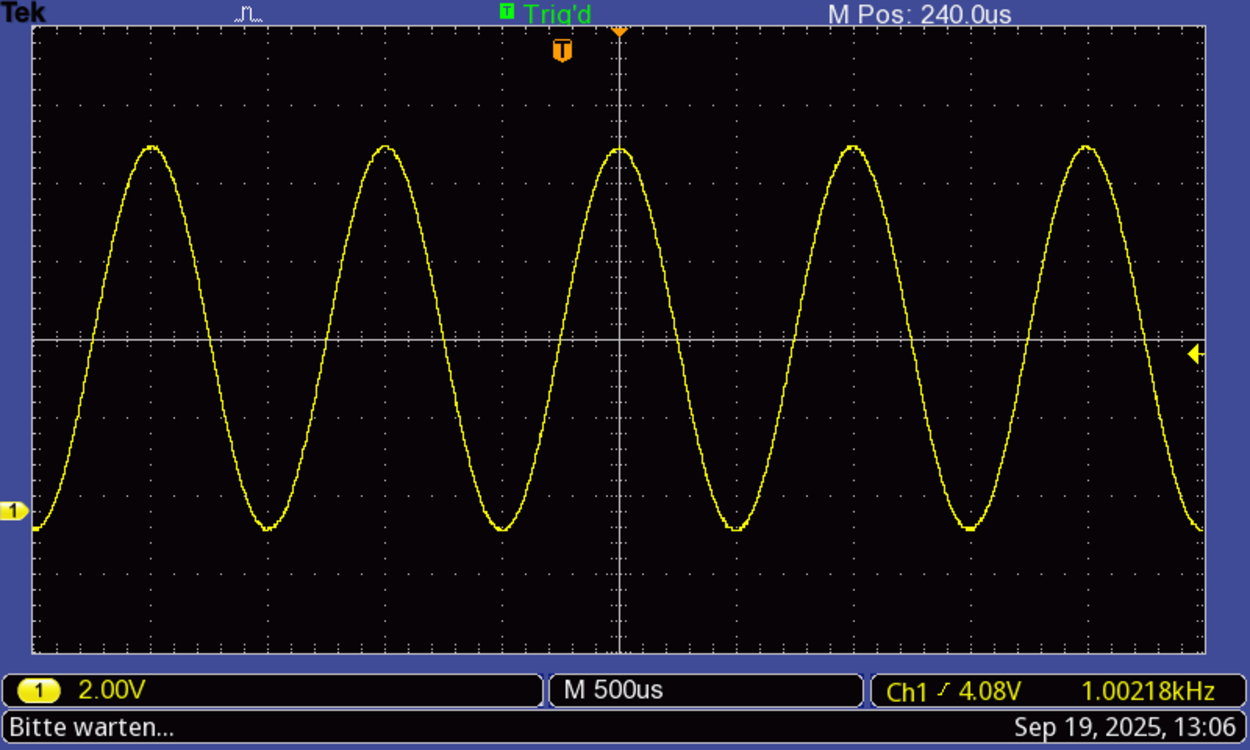
\includegraphics[width=0.45\textwidth]{img/25/Signale2/Signal4.pdf}
    \caption{Signal 4}
\end{figure}

Signal 4 ist wieder eine Sinus-Funktion.

\newpage

% ------------------- Signal 5 -------------------
\subsection*{Signal 5}

Für Signal 5 ist die Halbwertszeit zu bestimmen, also jene Zeit, bei der die Spannung um die Hälfte abgefallen ist.
Gemessen haben wir mit einer Divgröße von $500mV \times 2,5ms$ berechnet. Das Spannungsplatau lag bei $1V$. Wir haben also geschaut, wie groß die x-Achsen-Differenz vom Punkt, wo die Spannung abfällt, bis zu dem Punkt, an dem sie $500mV$ beträgt.

\begin{figure} [h!]
    \centering
        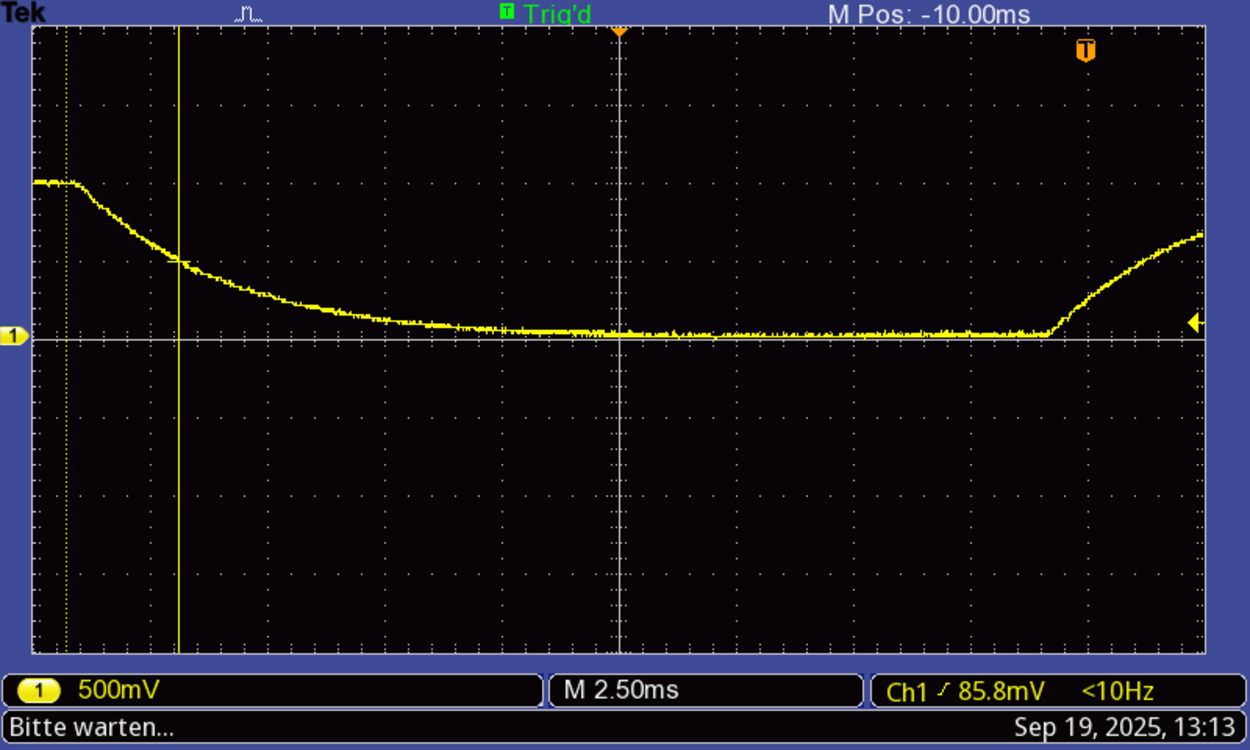
\includegraphics[width=0.45\textwidth]{img/25/Signale2/Signal5-Clean.pdf}
    \caption{Signal 5 nah rangezoomed um den Abfall klar zu erkennen.}
\end{figure}

Die Halbwertszeit liegt dabei bei 
\begin{equation}
    2,40 ms
\end{equation}.

Wir haben eine Auflösung von 2,5ms, wir haben also einen Zeitfehler von:
\begin{equation}
    0,16 ms
\end{equation}

Wir tragen das gesamte zu einem Ergebnis zusammen:
\begin{equation}
\boxed{
    t_H = (2,40 \pm 0,16)\, ms
}
\end{equation}


Außerdem sind hier nochmal die beiden Grafiken, die zum Vergleich der AC und der DC-Spannung dienen. Abbildung \ref{fig:sig5-ac} zeigt die AC-Spannung, Abbildung \ref{fig:sig5-dc} die DC-Spannung.
\onecolumn
\begin{figure} [h!]
    \centering
        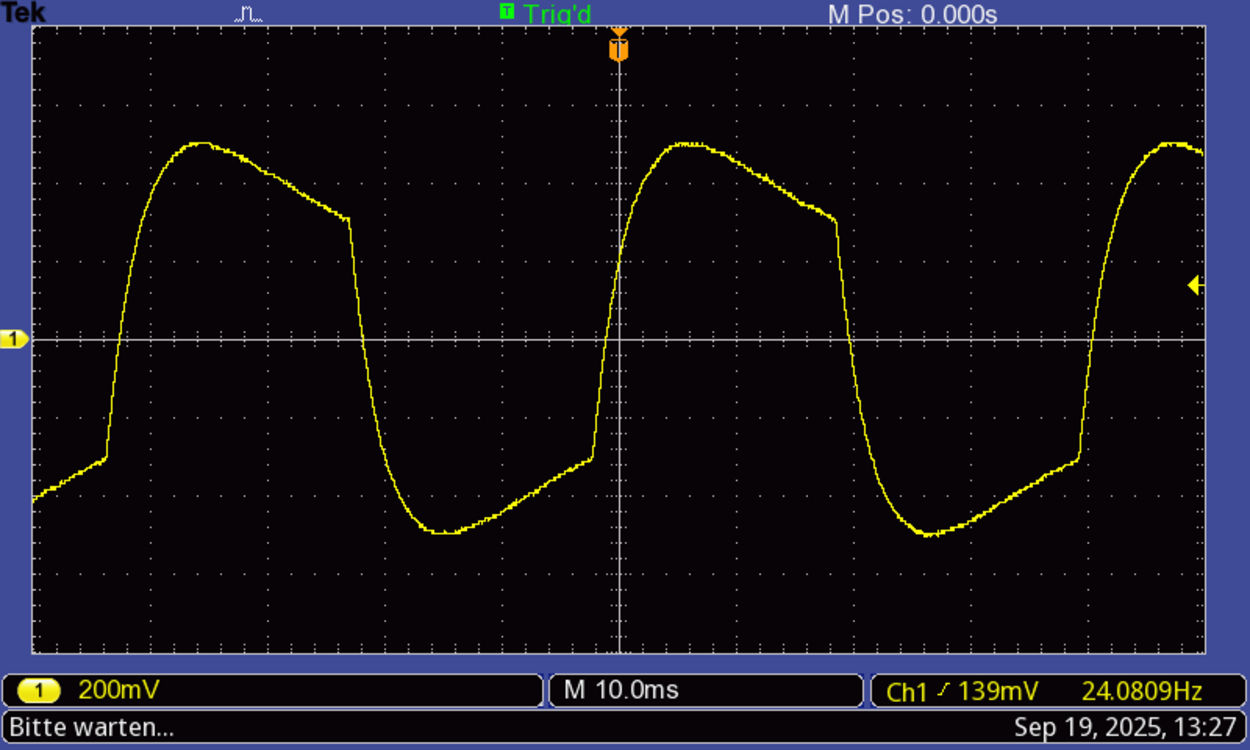
\includegraphics[width=0.8\textwidth]{img/25/Signale2/Signal5-AC.pdf}
    \caption{Signal 5-AC modus}
    \label{fig:sig5-ac}
\end{figure}

\begin{figure} [h!]
    \centering
        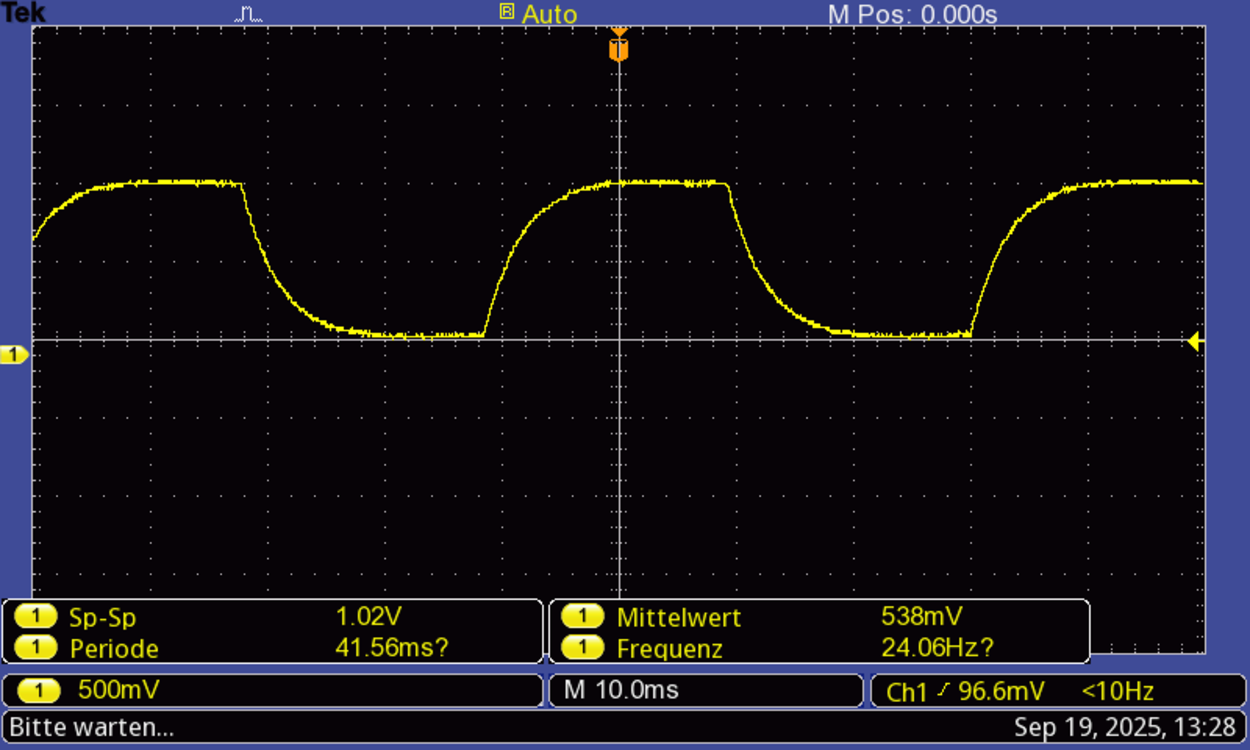
\includegraphics[width=0.8\textwidth]{img/25/Signale2/Signal5-DC.pdf}
    \caption{Signal 5-DC Modus}
    \label{fig:sig5-dc}
\end{figure}
\twocolumn

\newpage
\onecolumn
\twocolumn

% ------------------- Signal 6 -------------------
\subsection*{Signal 6}
\begin{figure} [h!]
    \centering
        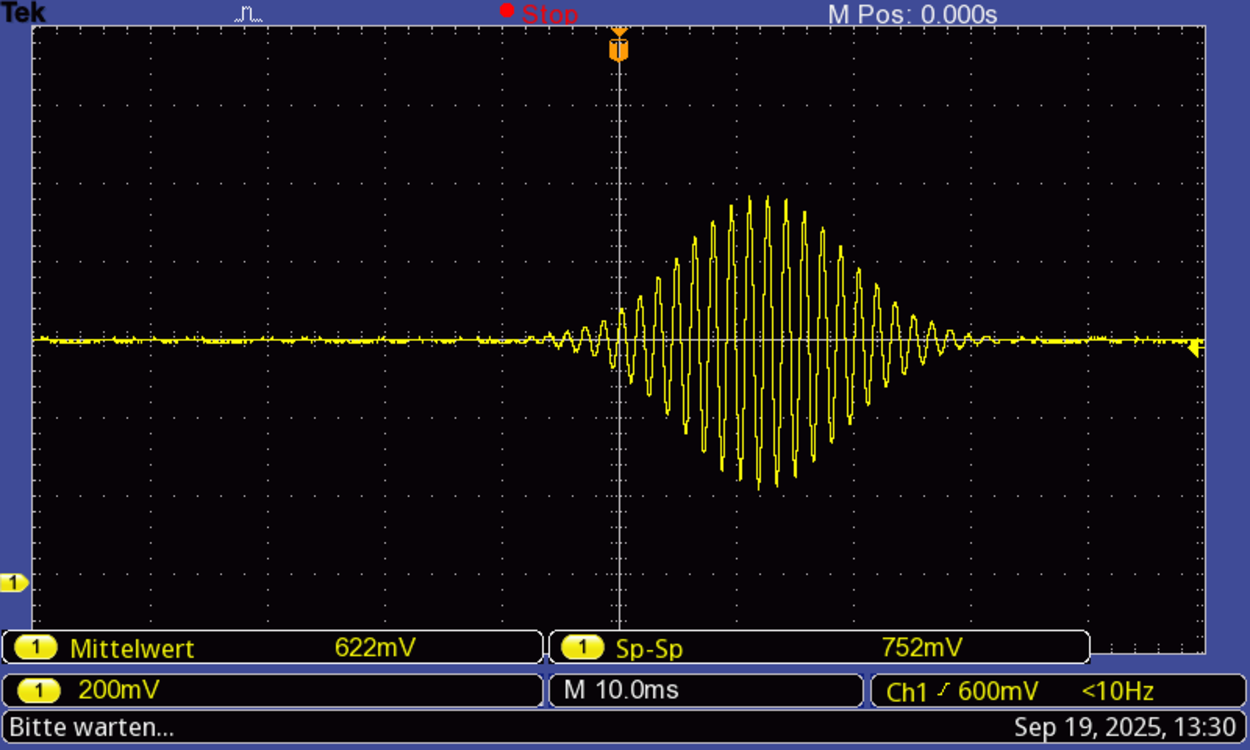
\includegraphics[width=0.45\textwidth]{img/25/Signale2/Signal6.pdf}
    \caption{Signal 6}
\end{figure}

% ------------------- Signal 7 -------------------
\subsection*{Signal 7}
\begin{figure} [h!]
    \centering
        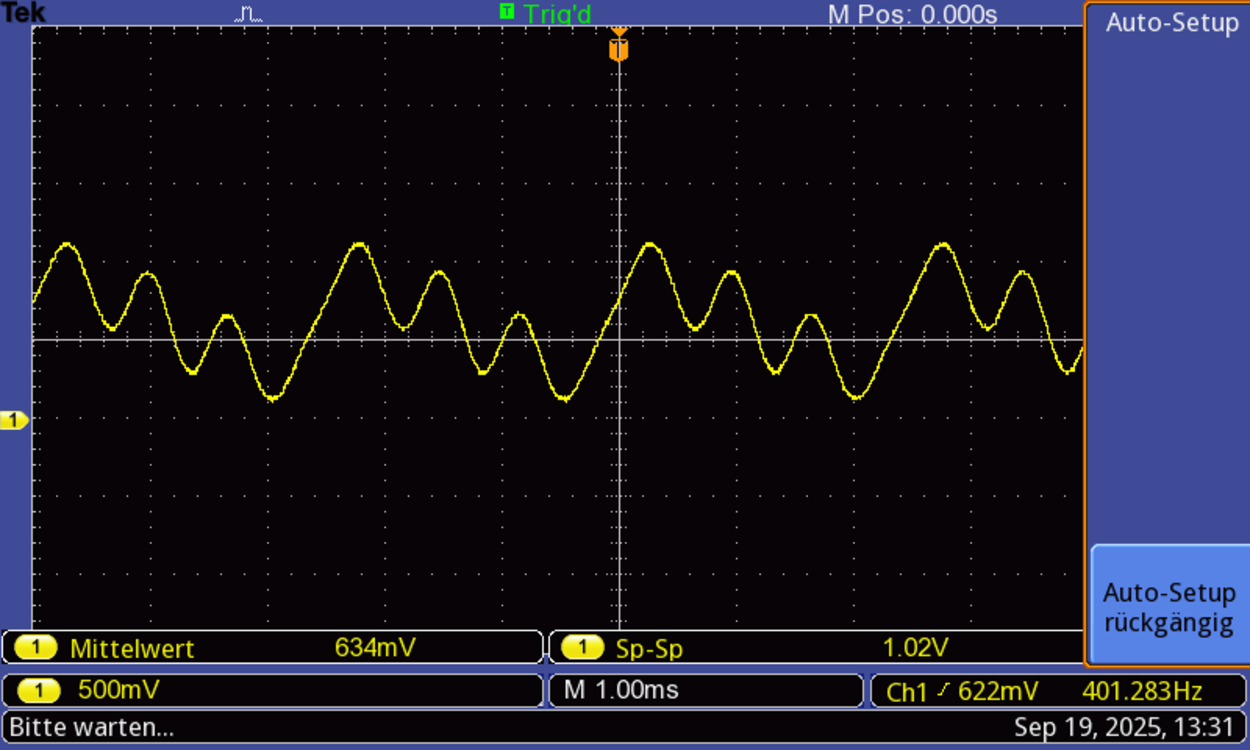
\includegraphics[width=0.45\textwidth]{img/25/Signale2/Signal7.pdf}
    \caption{Signal 7}
\end{figure}

\newpage

% ------------------- Signal 8 -------------------
\subsection*{Signal 8}
\begin{figure} [h!]
    \centering
        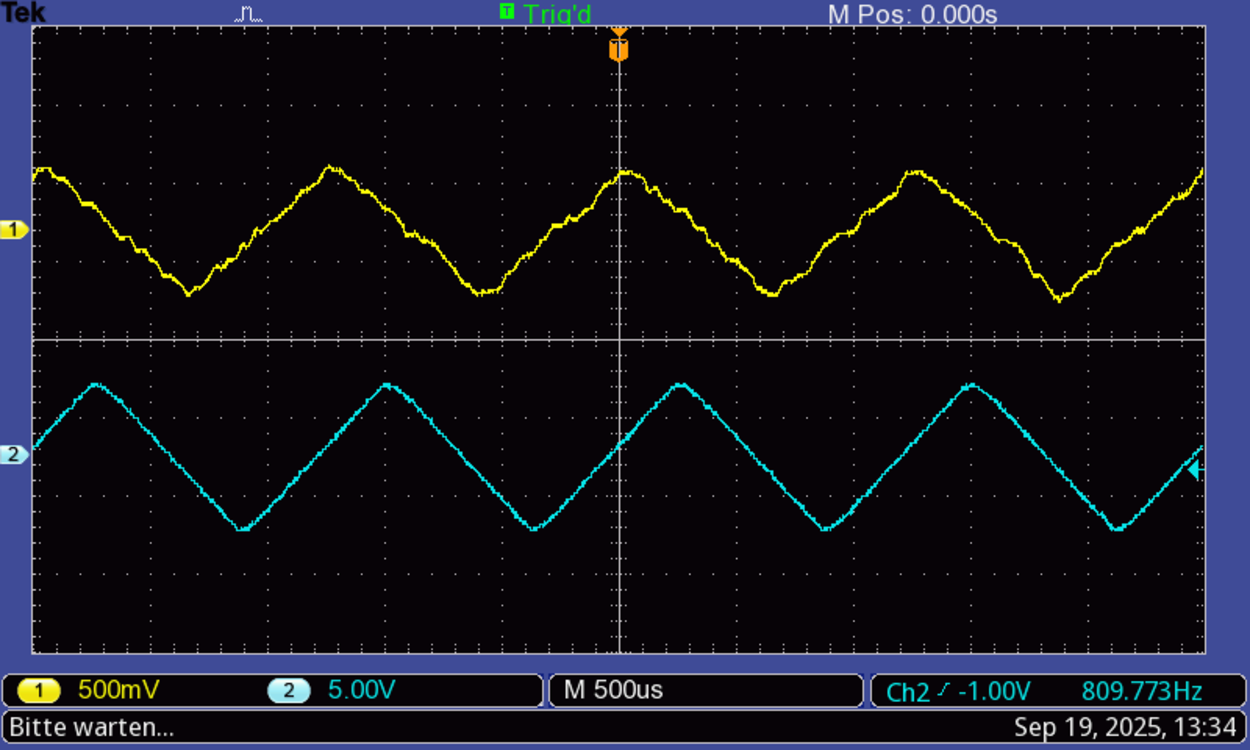
\includegraphics[width=0.45\textwidth]{img/25/Signale2/Signale8-deutlich-getrennt.pdf}
    \caption{Signal 8 mit verschobenen Nullpunkten und verschiedenen Amplituden.}
\end{figure}

\begin{figure} [h!]
    \centering
        \includegraphics[width=0.45\textwidth]{img/25/Signale2/Signale8-Überlagerung.pdf}
    \caption{Signal 8 mit gleichem Nullpunkt, aber verschiedenen Amplituden.}
\end{figure}

\newpage 

% ------------------- Signal 9 -------------------
\subsection*{Signal 9}

Für Signal 9 sind wieder Messungen betrieben wurden. D
\begin{figure} [h!]
    \centering
        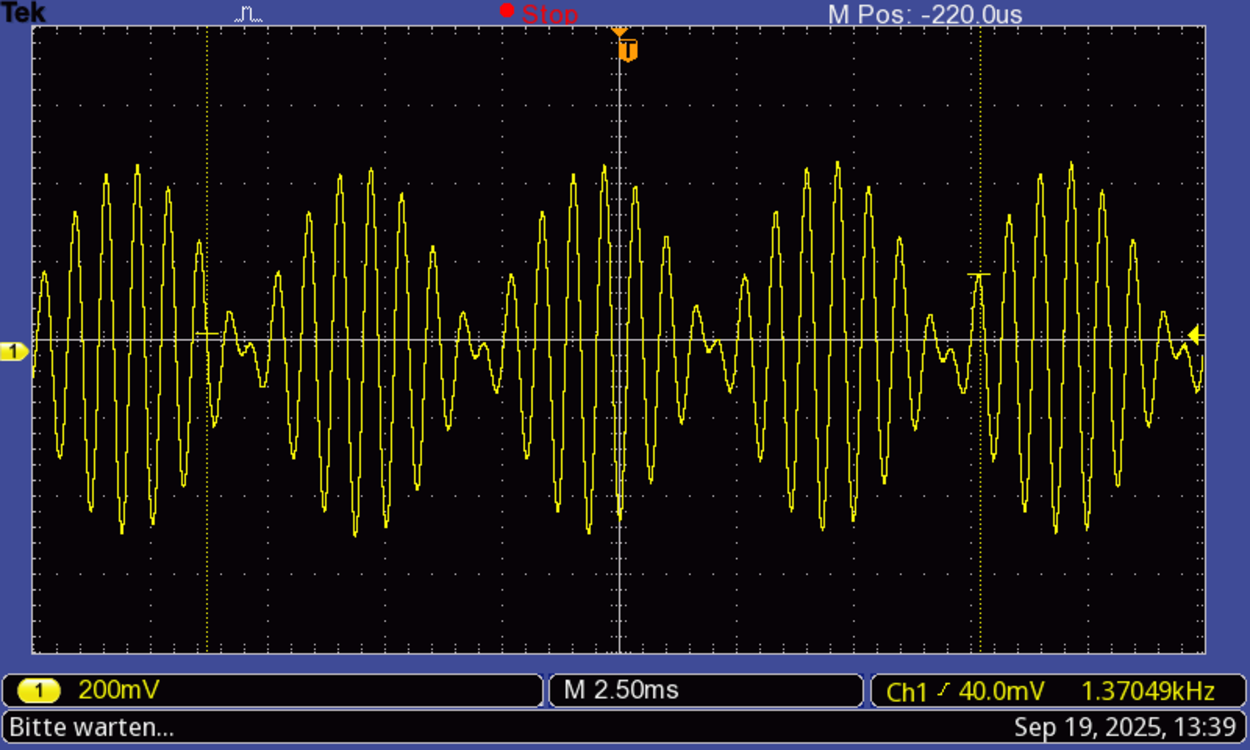
\includegraphics[width=0.45\textwidth]{img/25/Signale2/Signal9-Gesamt.pdf}
    \caption{Signal 9. Man sieht die Pahsen und die Gruppen sehr gut}
\end{figure}

\begin{figure} [h!]
    \centering
        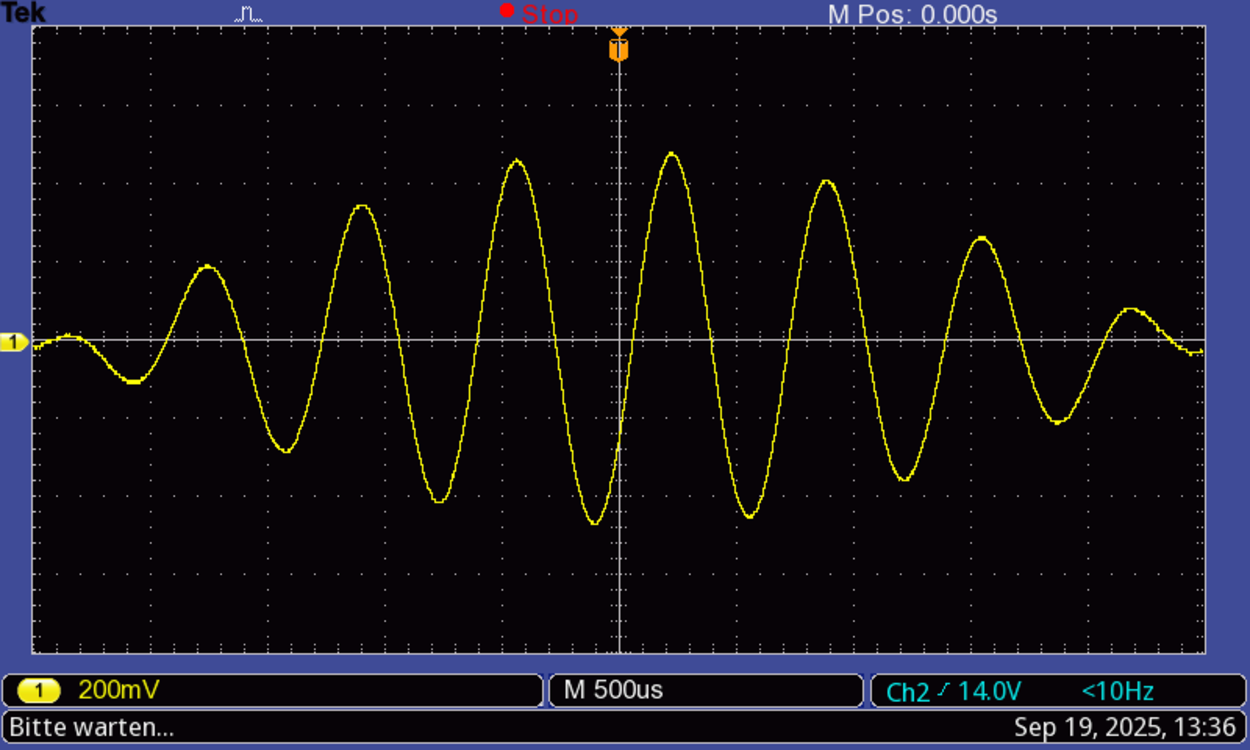
\includegraphics[width=0.45\textwidth]{img/25/Signale2/Signal9-einzeln.pdf}
    \caption{Signal 9, einzelne Gruppe.}
\end{figure}

\begin{figure} [h!]
    \centering
        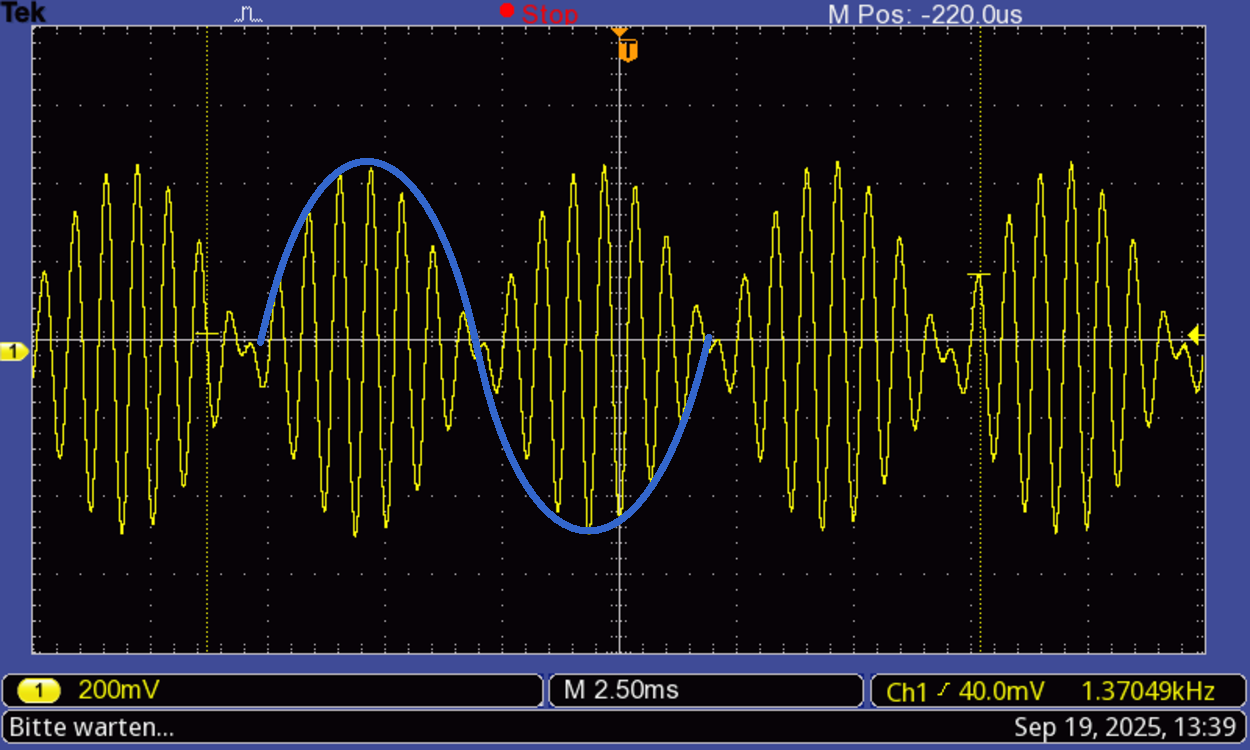
\includegraphics[width=0.45\textwidth]{img/25/Signale2/Signal9-Sin-eingezeichnet.pdf}
    \caption{Signal 9, eingezeichnete Phase.}
\end{figure}

\begin{figure} [h!]
    \centering
        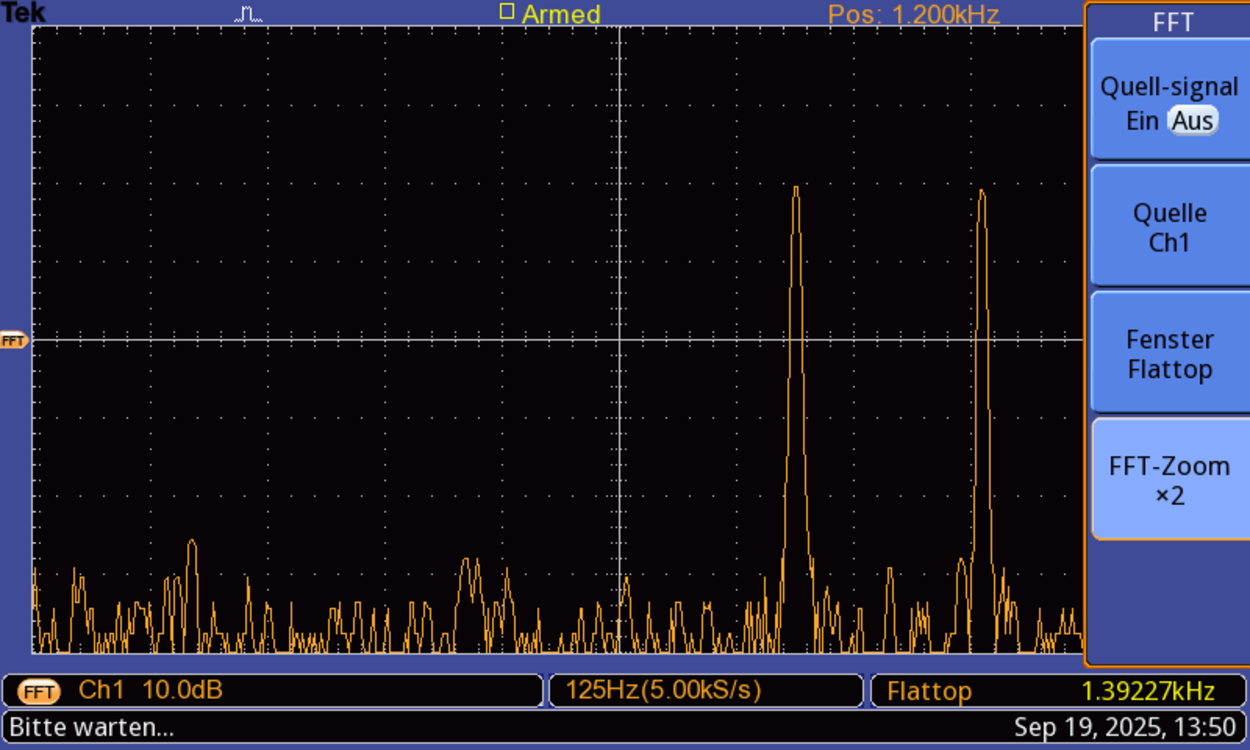
\includegraphics[width=0.45\textwidth]{img/25/Signale2/Sig9-FFT.pdf}
    \caption{Signal 9, eingezeichnete Phase.}
\end{figure}



\newpage
\onecolumn
\twocolumn


% ////////////  Aufgaben Wechsel ////////////
\section{Aufgabe 3: Pulsweitenmodulation}

% ////////////  Aufgaben Wechsel ////////////
\section{Aufgabe 4: Koaxialkabel}